\documentclass[12pt]{article}
\usepackage[utf8]{inputenc}
\usepackage[T2A]{fontenc}
\usepackage[russian]{babel}
\usepackage{amsmath}
\usepackage{amssymb}
\usepackage{dsfont}
\usepackage[dvipsnames]{xcolor}
\usepackage{setspace}
\usepackage{multirow}
\usepackage[a4paper, outer=1.5cm, inner=1.5cm, top=1cm, bottom=1cm]{geometry}
\usepackage{graphicx}
\usepackage{skull}
\usepackage{wasysym}
\usepackage{float}
\graphicspath{{.images/}}
\usepackage{hyperref}
\hypersetup{colorlinks=true, linkcolor=blue, filecolor=magenta, urlcolor=cyan}
\usepackage[firstpage]{draftwatermark}
\SetWatermarkText{
    $\qquad\qquad\qquad\qquad\qquad$\parbox{7cm}{\begin{center}
    
\includegraphics[width = 0.08\textwidth]{lion-logo.png}\bigskip\\~\bigskip\\~\vspace{-24mm}\\~\end{center}}
}
\SetWatermarkAngle{0}
\SetWatermarkScale{1.5}
\usepackage{etoolbox}

\newtoggle{ifsolved}
\newtoggle{needhelp}
\newcounter{num}
\setcounter{num}{1}

\newcommand{\newnum}{\par\textbf{\textnumero\arabic{num}}\stepcounter{num}}
\newcommand{\sol}{\vspace{3mm}\par\textbf{Решение: }}
\newcommand{\ans}{\vspace{3mm}\par\textbf{Ответ: }}
\newcommand{\hint}{\vspace{3mm}\par\textbf{Подсказка: }}
\newcommand{\mode}[1]{
\ifstrequal{#1}{0}{\togglefalse{ifsolved}\togglefalse{needhelp}}{\ifstrequal{#1}{1}{\togglefalse{ifsolved}\toggletrue{needhelp}}{\ifstrequal{#1}{2}{\toggletrue{ifsolved}\togglefalse{needhelp}}{\toggletrue{ifsolved}\toggletrue{needhelp}}}}} %if 0 - if 1 - if 2 - else
%\newenvironment{problem}[8]{%#1, #2, #3
%\parbox{\linewidth}{\vspace{4mm}\ifstrequal{#4}{(лёгкая)}{\newnum\textbf{.}}{\newnum\textbf{*.} } \\ #5}
%\iftoggle{ifsolved}{\sol #6}{}
%\iftoggle{ifsolved}{\ans #7}{}
%\iftoggle{needhelp}{\hint #8}{}}

\newenvironment{problem}[8]{%#1, #2, #3
\parbox{\linewidth}{\vspace{5mm}\ifstrequal{#4}{(лёгкая)}{\newnum\textbf{.}}{\newnum\textbf{*.} } \\ #5}
\iftoggle{ifsolved}{\sol #6}{}

\iftoggle{ifsolved}{\parbox{\linewidth}{\ans #7}}{}
\iftoggle{needhelp}{\parbox{\linewidth}{\hint #8}}{}}

\newenvironment{mylist} %custom list
{ \begin{itemize}
    \setlength{\itemsep}{0pt}
    \setlength{\parskip}{0pt}
    \setlength{\parsep}{0pt}     }
{ \end{itemize}                  }

\newenvironment{homeass}[1]{\vspace*{-1.5cm}
\iftoggle{ifsolved}{
    \section*{\center{Решение домашнего задания к #1.}}
}{
    \section*{\center{\textcolor{Sepia}{Домашнее задание к #1}}}
} \vspace{7mm}\large}

\parindent=0pt
\pagestyle{empty}
%$\!$[\arabic{class}.\arabic{num}]
%\ifnumcomp{\value{counter}}{>}{1}{true}{false}
%\definecolor{Gray}{gray}{0.9}
%\definecolor{mypink}{RGB}{219, 48, 122}
%\newcolumntype{g}{>{\columncolor{Gray}}p{2.8cm}}

\begin{document}
\large
\mode{7}
%0 for problems without hints
%1 for problems + hints
%2 for problems + solutions + answers
%else: show all

{\centering\section*{СПИСОК ЗАДАЧ}}

{\centering\subsection*{\smallskip\\\textcolor{green}{\textbf{Полезные вещи, которые можно и нужно копипастить:}}}}

\subsection*{\textcolor{Emerald}{\textbf{Полезные шпаргалки по LaTeXу:}}}

\textbf{Пример вставки рисунка:}

\begin{minipage}{\linewidth}
    \begin{minipage}{0.54\linewidth}
    см. рисунок справа\\
    Текст к собственно пикче, примерно всегда это либо развёрнутое описание, либо большая часть решения задачи --- стремимся экономить пространство, если это можно сделать.
    \end{minipage}
    \hspace{0.05\linewidth}
    \begin{minipage}{0.4\linewidth}
    \begin{figure}[H] 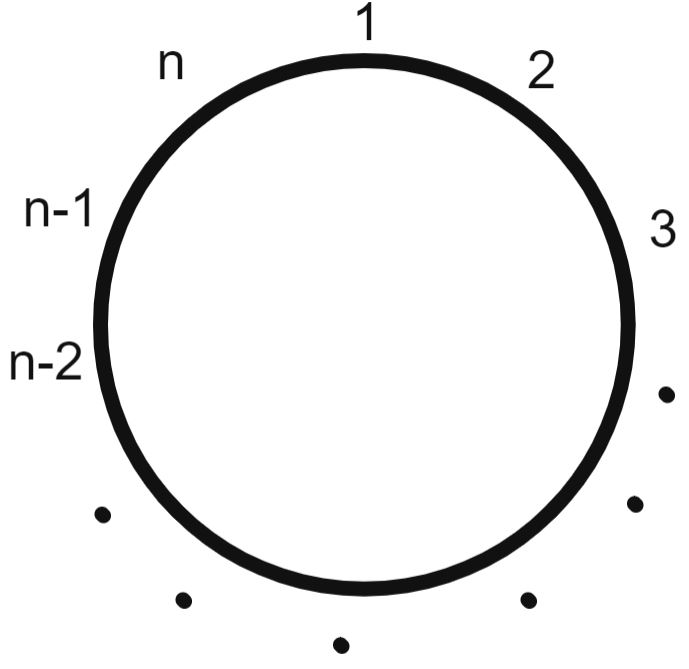
\includegraphics[width=\linewidth]{sol3} %тут поменять имя пикчи
    \end{figure}
    \end{minipage}
\end{minipage}

\textbf{Дефолтные математические знаки и символы:}\\
$\geqslant$,
$\leqslant$,
$a^{b}$,
$x_{i}$,
$\sqrt{a}$,
$\frac{a}{b}$,
$\displaystyle \frac{a}{b}$,
$\cdot$
$\;\Rightarrow\;$,
$\;\Leftrightarrow\;$,
$1{,}2$.
О промежутках:
$a\!b$,
$a\,b$,
$a\:b$,
$a\;b$,
$a\quad b$.

\textbf{Стандартные система и совокупность уравнений / неравенств:}\\
$\left\{
\begin{aligned}
f(x) &= 0 \\
g(x) &= 1
\end{aligned}\right.$

$\left[\begin{aligned}
&\left\{\begin{aligned}
f(x) &\geqslant a \\
g(x) &= b
\end{aligned}\right.\\
&\left\{\begin{aligned}
f(x) &< a \\
g(x) &= -b
\end{aligned}\right.
\end{aligned}\right.$

\subsection*{\textcolor{Emerald}{\textbf{Не математическое, но полезное:}}}
% комментарий в любом месте документа, который нигде не будет видно. Можно использовать для написания заметок-вопросов по задачам
\textbf{Пример таблицы:}

\begin{tabular}{|c|c|c|}
\hline
    $a$ & $b$ & текст
\\\hline
    $c$ & $d$ & мораль
\\\hline
\end{tabular}\\

\textbf{Отступы:} между\smallskip\\ строками\medskip\\ \textbf{Тире} --- это три дефиса.\\
\textbf{Списки:}
\begin{mylist}
\item [$\bullet$] это был пункт а
\item [2)] а это уже пункт номер 2 с изменённым заголовком
\end{mylist}

\subsection*{\textcolor{Emerald}{\textbf{Всё, неупомянутое выше (или если просто что-то не так):}}}
\begin{mylist}
\item [$\bullet$] Решение отдельных вопросов касательно ТеХа нужно искать в \href{https://www.mccme.ru/free-books/llang/newllang.pdf}{Львовском}.

\item [$\bullet$] Найти произвольный символ, который нужен, можно в \href{http://detexify.kirelabs.org/classify.html}{Detexify}.

\item [$\bullet$] Если возникли сомнения при решении, ответ практически ко всем задачам можно проверить с помощью \href{https://www.wolframalpha.com/}{WolframAlpha}.

\item [$\bullet$] Если в задаче нужно создать картинку, то лучше пока отложить эту задачу. Все графики планируется централизованно нарисовать (или перерисовать) в геогебре.

\item [\textcolor{brown}{\textbf{!!}}] Важно ставить \textcolor{red}{\textbf{$\spadesuit$}}
(или просто red) в тело задачи в случае серьёзных вопросов к решению и какой-то вопиющей лажи.

\item [\textcolor{brown}{\textbf{!!}}] Важно ставить \textcolor{olive}{\textbf{$\spadesuit$}}
(или просто olive) в тело задачи в случае не самого удачного текста и кривых отступов.
\end{mylist}

\subsection*{\textcolor{Violet}{\textbf{Комментарии:}}}% а также невидимые комментарии - так можно оставлять заметки-вопросы прямо в задаче, чтобы потом было понятно, в чём вопрос.
\begin{mylist}
\item [$\skull$] Переставлять задачи местами --- очень плохая идея.

\item [$\smiley$] При двойном клике по тексту pdf справа происходит автоматический переход к этому месту в латех-коде, а для обратного перехода можно нажать стрелку вправо (висит сверху между pdf и латех-кодом).

\item [$\smiley$] Если есть размышления, дописывать red/olive к задаче или не дописывать, то лучше всё-таки дописать.

\item [$\skull$] Самое плохое, что можно сделать --- написать в любое поле из трёх (НаписанноеРешение/ВерныйОтвет/Подсказка) только половину того, что надо, никак это не отметить, и потом пойти дальше.\\ Нужно в этот момент писать red/olive в случайном месте задачи, чтобы потом вычислить это с помощью Ctrl+F по всему документу (и это то, что потом будет делаться долго и тщательно)
\end{mylist}

\newpage
\setcounter{num}{573}

\hypertarget{7.3}{{\centering\section*{\bigskip\\\textcolor{Blue}{\hyperlink{start2}{\textcolor{Blue}{7.3}} Степень с натуральным показателем.}\vspace{-5mm}}}}

\begin{problem}{Свойства степени с натуральным показателем.}{7.3.3}{6K}{(лёгкая)}
{Найти $z$, являющийся решением уравнения: $\;\displaystyle 2 \cdot \frac{4}{5} \cdot \frac{5}{z} = z^{2}$.}
{Перемножим всё в левой части уравнения. Получаем, что $\displaystyle \frac{8}{z} = z \cdot z$.\smallskip\\ Несложно подметить, что $z \neq 0$, так как делить на 0 нельзя. Поэтому домножим на $z$ обе части уравнения (и слева, и справа станет в $z$ раз больше, а значит уравнение сохранится). Поэтому $\frac{8}{z} \cdot z = z \cdot z \cdot z$, то есть $2 \cdot 2 \cdot 2 = z \cdot z \cdot z$.\\ Теперь мы можем сразу сказать, что тут есть решение: $z = 2$. Также понятно, что нельзя взять $z$ ни меньше, ни больше, то есть никаких других решений тут нет.}
{Данное уравнение имеет решение $z = 2$.}{Домножить обе части уравнения на $z$~--- хорошая идея.}
\end{problem}

\begin{problem}{Свойства степени с натуральным показателем.}{7.3.3}{6K}{*}
{Решить уравнение и найти $x$: $\;\displaystyle\vphantom{\rule{0pt}{18pt}}\frac{4}{5} \cdot \frac{9}{5} = x \cdot x$.}
{Перемножим дроби. Получаем, что $\displaystyle x \cdot x = \frac{36}{25}$.\smallskip\\ Несложно догадаться, что для того, чтобы получить 36, нужно умножить 6 на 6, а чтобы получить 25~--- умножить 5 на 5. Поэтому логично сразу заявить, что одно решение мы знаем: это $ x = \frac65$. Однако, если вспомнить про правило <<минус на минус даёт плюс>>, то становится понятным, что есть и второе решение, $ x = -\frac65$. Таким образом, решений два, $ x = \frac65$ и $ x = -\frac65$.}
{Решений у данного уравнения два: $x = \pm \frac65$.}{<<Минус на минус даёт плюс>>.}
\end{problem}

\begin{problem}{Свойства степени с натуральным показателем.}{7.3.3}{6K}{(лёгкая)}
{Найти значение выражения $(a + b)^{4}$, если $a = 1{,}4$, $\,b = -1{,}5$.}
{НаписанноеРешение}
{ВерныйОтвет}{Подсказка}
\end{problem}

\begin{problem}{Свойства степени с натуральным показателем.}{7.3.3}{6K}{(лёгкая) \textcolor{olive}{\textbf{$\spadesuit$}}}
{\vspace{-3mm}\\\begin{minipage}{\linewidth}
    \begin{minipage}{0.58\linewidth}
    На координатной прямой отметили числа $a$ и $b$. Какие из приведённых ниже утверждений~--- ложны?
    \\a) $\;ab > 0$; \hfill b) $\;a^{2} b^{3} > 0$;\,
    \\c) $a - b > 0$; \hfill d) $a + b > 0$.
    \end{minipage}
    \hspace{0.02\linewidth}
    \begin{minipage}{0.4\linewidth}
        \begin{figure}[H]
        
\includegraphics[width=\linewidth]{6K-12}
        \end{figure}
    \end{minipage}
\end{minipage}}
{Из рисунка видно, что $a > 0$, а $b < 0$. Произведение положительного и отрицательного числа отрицательно, следовательно пункт а) неверен.\\ При этом, поскольку $a^2$ положительное число, а $b^3$ отрицательное, $a^2b^3$~--- отрицательное число, и пункт b) тоже неверен.\\ Теперь пункт с). $a - b$~--- это положительное число минус отрицательное число, результат является положительным числом. Поэтому с)~--- верное утверждение.\\ Из рисунка видно, что $|a| < |b|$. Следовательно, так как $b$~--- отрицательное число, $a + b$ отрицательно, и утверждение $d)$ неверно. Итого ложно всё, кроме $c)$.}
{Ложными утверждениями являются a), b), d). (все, кроме с))}{Какой знак имеет произведение двух чисел с разными знаками?}
\end{problem}

\begin{problem}{Свойства степени с натуральным показателем.}{7.3.3}{6K}{(лёгкая)}
{Известно, что $a > 0$, а $c < 0$. Сравнить с нулём значение выражения $a^{3} c^{4}$.
\\a) $a^{3} c^{4} < 0$; \hfill b) $a^{3} c^{4} > 0$; \hfill c) $a^{3} c^{4} = 0$; \hfill d) Это невозможно.}
{Поскольку $a$ положительно, $a^3$ также положительно. $c$ отрицательно, а значит $c^4$ положительно (минус на минус даёт плюс). Произведение $a^3$ и $c^4$~--- двух положительных чисел~--- положительно. Правильный ответ~--- $b)$.}
{$a^{3} c^{4} > 0$. Верный ответ~--- b).}{Какой знак у произведения отрицательных чисел?}
\end{problem}

\begin{problem}{Свойства степени с натуральным показателем.}{7.3.3}{6K}{(лёгкая)}
{В этой задаче нам известно, что $a$~--- число положительное, а $b$~--- отрицательное. Значение какого из выражений, написанных ниже, больше всех остальных?
\\ \hfill a) $\displaystyle\frac{b}{a}$; \hfill b) $\displaystyle -\frac{a}{b^{2}}$; \hfill c) $\displaystyle\frac{a^{2}}{b}$; \hfill d) $\displaystyle\frac{a^{2}}{b^{2}}$}
{НаписанноеРешение}
{ВерныйОтвет}{Подсказка}
\end{problem}

\begin{problem}{Свойства степени с натуральным показателем.}{7.3.3}{6K \textcolor{red}{\textbf{$\spadesuit$}} второе отправить в многочлены, первое оставить}{*}
{a) Рассмотрим следующее выражение: $D = x^{2} - 4$.\\ Насколько маленьким оно может быть? Почему?
\\b)* А выражение $R = x^{2} + 2x + 3$? Почему?}
{НаписанноеРешение}
{ВерныйОтвет}{Подсказка}
\end{problem}

\begin{problem}{Свойства степени с натуральным показателем.}{7.3.3}{6K}{*}
{Найти последнюю цифру числа: 
\\a) $3^{5}$; \hfill b) $3^{44}$; \hfill c) $3^{333}$.}
{Начнём с пункта а). $3^1 = 3$, $3^2 = 3\cdot3 = 9$, $3^3 = 3^2\cdot3 = 9\cdot3 = 27$, $3^4 = 3^3\cdot3 = 27\cdot3 = 81$, $3^5 = 81\cdot3 = 243$. Последняя цифра этого числа~--- 3.\smallskip\\
b) Логично, что последняя цифра будет каждый раз нечётной (но не пятёркой).\\
Посмотрим на несколько следующих степеней: $3^6 = 3^5\cdot3 = 243\cdot3 = 729$, $3^7 =\\= 3^6\cdot3 = 729\cdot3 = 2187$. Можно заметить, что последние цифры повторяются в следующем порядке: 3, 9, 7, 1, 3, 9, 7, 1, ... и таким образом, поскольку $3^{44} = (3^4)^{11}$, цикл повторится ровно 11 раз. В итоге мы остановимся на 1, то есть последней цифрой числа $3^{44}$ будет 1.\smallskip\\
c) Нужно понять, сколько раз в 333 входит наш цикл из четырёх цифр.\\ Для этого поделим 333 на 4 с остатком: $333 : 4 = 83$ (ост. 1) Это означает, что мы 83 раза пройдём цикл из этих 4 цифр, а следующее число будет первым в очередной четвёрке, и его последняя цифра будет последней цифрой числа $3^{333}$.\\
То есть, последняя цифра в данном случае~--- 3.}
{$3^5$ оканчивается на 3, $\,3^{44}$ оканчивается на 1, $\,3^{333}$ оканчивается на 3.}{Последние цифры циклически повторяются.}
\end{problem}

\begin{problem}{Свойства степени с натуральным показателем.}{7.3.3}{6K}{*}
{Найти последнюю цифру числа: 
\\a) $2^{1}$; \hfill b) $2^{12}$; \hfill c) $2^{123}$.}
{НаписанноеРешение}
{ВерныйОтвет}{Подсказка}
\end{problem}

\begin{problem}{Свойства степени с натуральным показателем.}{7.3.3}{6K}{*}
{Сумма нескольких чисел (возможно одинаковых, возможно нет) равна 1.\\ Может ли быть такое, что сумма квадратов этих же чисел равна: 
\\ \hfill a) $\frac{1}{2}$?\hfill b) $\frac{1}{3}$? \hfill c) $0{,}01$?\hfill d) $5$?? \hfill}
{a) Берём две половины: $\frac12 + \frac12 = 1$, и $\left(\frac12\right)^2 + \left(\frac12\right)^2 = \frac24 = \frac12$. Может.\\
b) Берём три трети: $\frac13 + \frac13 + \frac13 = 1$, и $\left(\frac13\right)^2 + \left(\frac13\right)^2 + \left(\frac13\right)^2 = \frac39 = \frac13$. Может.\\
с) Берём $\frac{1}{100}$: $\;\frac{1}{100} + \ldots + \frac{1}{100} = 1$, и $\left(\frac{1}{100}\right)^2 + \ldots + \left(\frac{1}{100}\right)^2 = \frac{100}{10000} = 0{,}01$. Может.\\
d) Этот пункт отличается от предыдущих. Возьмём числа $2$ и $-1$. $\;2 + (-1) = 1$. $2^2 + (-1)^2 = 4 + 1 = 5$. Таким образом, все варианты возможны.}
{Возможно всё~--- возведение в квадрат не обязательно увеличивает число.

}{Во всех пунктах, кроме последнего, можно брать равные числа.}
\end{problem}

\end{document}